\section{Iteration 2: Decomposition of the Remote Module Communication Unit}
\label{add:it2}

\subsection{Step 1: Identify candidate drivers}
\label{add:it2/drivers}

\npar In the previous iteration, four quality attributes (Av2', M1', M2' and
M3') and three use cases (UC7, UC8' and UC13') were assigned to the remote
module communication unit and 2 use cases (UCx and UCy) were created. 

\npar There is no real coupling between the quality attributes and the use cases
so the following quality attributes will form the drivers for this
iteration:

\begin{itemize}
  \item Av2': Missing measurements.
  \begin{itemize}
    \item When a measurement did not arrive this should be logged, when
  this happens for the third time a ReMes Operator should be notified. This
  detection should occur in less than ten minutes.
	\item Trames should be resent when their receival deadline is elapsed.
  \end{itemize}
  \item M1': Dynamic pricing.
  \begin{itemize}
    \item New types of remote devices will be introduced (with possibly new
    data formats of the trames they send).
  \end{itemize}
  \item M2': Fine-grained metering for enterprises.
  \begin{itemize}
    \item The secondary meters can introduce new trame formats.
  \end{itemize}
  \item M3': Decentralized electricity generation
  \begin{itemize}
    \item The production meters could define a new trame format.
  \end{itemize}
\end{itemize}

\npar The use cases delegated to this unit are given below.

\begin{itemize}
	\item UC7 : Send trame to remote device.
	\item UC8': Send measurement.
	\begin{itemize}
    	\item ReMeS is responsible for customer accounting information
    	\item Remote modules are marked as active when they send their first
    	trame.
  	\end{itemize}
  	\item UC13': Send alarm.
  	\begin{itemize}
		\item %TODO
  	\end{itemize}
  	\item UCx: Retrieve customer from trame.
  	\item UCy: Retrieve remote module protocol.
\end{itemize}

\subsection{Step 2: Choose design concepts}
\label{add:it2/concepts}

\subsubsection{Tactics}
\label{add:it2/tactics}

\paragraph{Modifiability}

\npar When opting for a modifiable solution 3 main (groups) of tactics can be
used: localize modifications, prevent ripple effect and defer binding time.
Two tactis are picked from the first group, namely abstraction of common
services and anticipate expected changes.

\npar To prevent rippling effects three tactics are employed. The first one,
probably the most important one, is the hiding of information through the use of
interfaces. Furthermore are communication paths restricted and an intermediary
will be used.

\paragraph{Availability}

\npar The chosen availability tactic is detection, more specific the heartbeat
mechanism.

\subsubsection{Design Patterns}
\label{add:it2/patterns}

\npar To realize the modifiability tactics and allow the coverage of UC7', the
\emph{Message Translator} pattern is selected. The translator acts an
intermediary between the remote module and ReMeS and all information remains
hidden behind a simple interface. 

\npar To push this information hiding even further a modified version of the
\emph{Resource Pool} pattern is used. This will be enlightened in the next
section.
%TODO: misschien is dit niet helemaal waar, want resource pool is meer op
% performantie gericht.

\npar Finally the \emph{Publisher - Subscriber} pattern is used to allow
multiple components to receive trames in parallel. 

\subsection{Step 3: Instantiate architectural elements and allocate responsibilities}
\label{add:it2/elements}

\begin{figure}[H]
	\begin{centering}
		% TODO Figure
		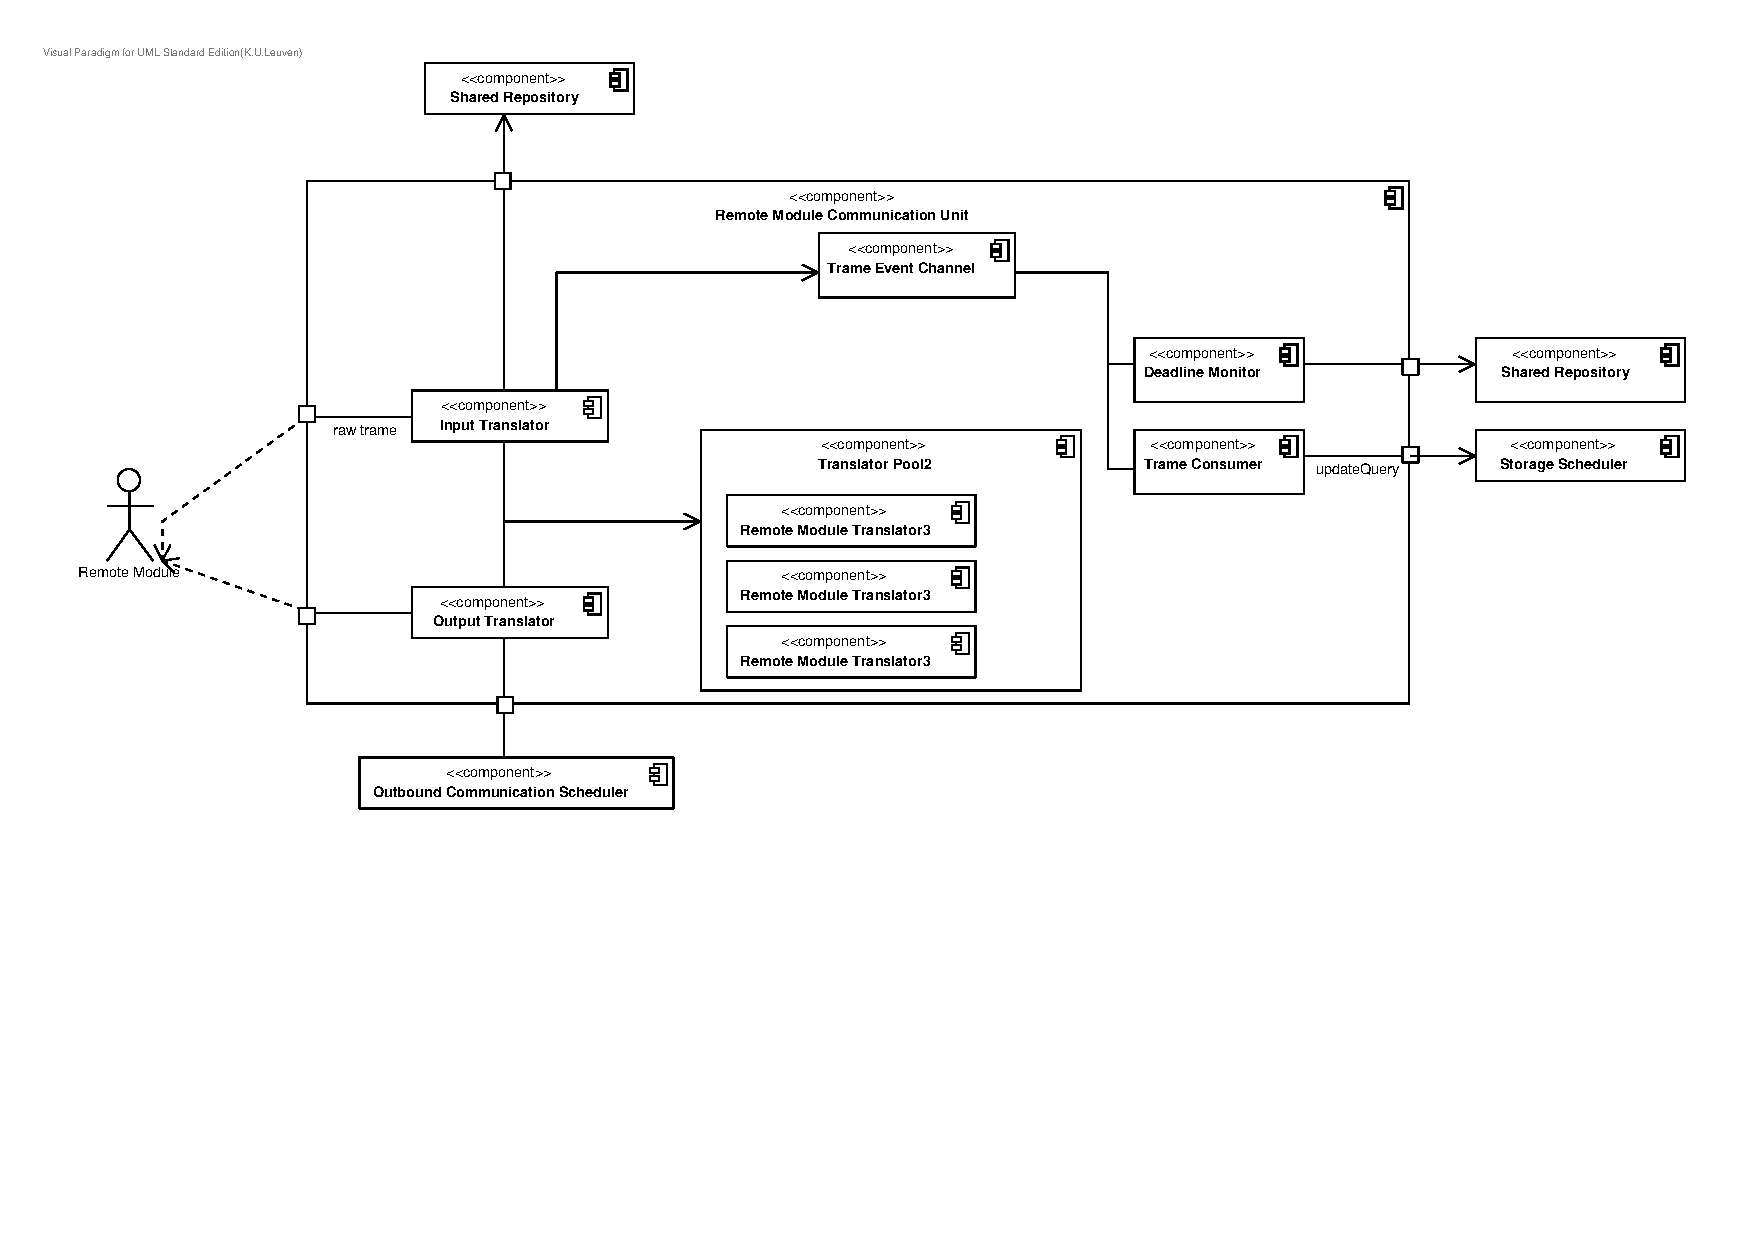
\includegraphics[width=\textwidth]{figs/add-it2-elements.pdf}
		\caption{Overview of the instantiated child elements in the Remote Module
		Communication Unit}
		\label{fig:it2/elements}
	\end{centering}
\end{figure}

\npar The remote module communication unit has three main components: Input
Translator, Output Translator, Translator Pool, Event Channel, Deadline Monitor
and Trame Consumer. Each of them will be discussed below. As one can see in
diagram \ref{fig:it2/elements} there are only two communication paths
in the system, one for incoming communication and one for outgoing. In this way
another tactic is realized, namely the restriction of communication paths.

\npar In the previous section there was the mentioning of a modified version of
the \emph{Resource Pool} pattern. One can see this pattern in the usage of the
translator pool. The translator pool component itself acts as a sort of manager
of the pool and handles incoming requests for translators based on a
certain module. The difference with the original pattern lies in the 
diversity of the translators. Each translator is different whereas the
resources normally should all be equal. 

\subsubsection{Input Translator}

\npar The input translator has as duty the translation of incoming (raw) trames
into objectified trames. Therefore it must know what the incoming data format
is. To realize this, it has a translator pool at its disposal where, based on
the module (type) a translator can be fetched. The translated trame is provided
with extra information concerning the customer (i.e. the owner of the module where the
trame came from). When the trames are translated they are published on the event
channel for all interested parties.

\subsubsection{Output Translator}

\npar This component is analogous to the input translator off course. This
component retrieves the right translator from the pool based on the module
where the incoming trame should be send to. It is important to notice that all
outgoing communication towards remote modules goes through this module.

\subsubsection{Translator Pool}

\npar The translator pool acts as the manager for the pool and all requests from
both the translators will pass through this component. 

\subsubsection{Event Channel}

\npar The event channel is the communication entity where publishers can publish
events on and subscribers can subscribe on.

\subsubsection{Deadline Monitor}

\npar The responsibility of this process is the monitoring of all bypassing
measurements and guaranteeing that a missing measurement is detected within the
demanded time limits. This monitor is subscribed to the event channel to receive
trames. To guarantee these limits the monitor keeps a table with expected
arrival times of all remote devices which is frenquently checked. Notice that to
protect from failures, this table is made persistent. When a deadline is
exceeded this is stored in the corresponding database. When a certain number of
deadline violations is reached a ReMeS operator is notified. Notice that this
component is in fact the realization of the heartbeat tactic. 

\subsubsection{Trame Consumer}

\npar The trame consumer is a simple forwarding unit which is subscribed to the
event channel and receives all trames which are published on it. It simply
forwards all trames to the storage scheduler.

\subsection{Step 4: Define interfaces for instantiated elements}
\label{add:it2/interfaces}

\subsubsection{Input Translator}

\paragraph{InputTrame}

\npar this interface was already discussed in iteration 1, see section
\ref{add:it1/interfaces}.

\subsubsection{Output Translator}

\paragraph{OutputTrame}

\npar this interface was already discussed in iteration 1, see section
\ref{add:it1/interfaces}.

\subsubsection{Translator Pool}

\paragraph{TranslatorManager}

\npar The translator pool interface offers one method,
\method{GetTranslatorFor(RemoteDevice)}. This method does nothing
else than return the correct translator for the given remote device (there can be
differences between remote module types, communication channels, etc.).

\paragraph{Translator}

\npar Each of the different translators implements the \interface{Translator}
translator interface. This interface includes two methods:
\method{translateFromDevice(RawTrame)} and
\method{translateToDevice(Message)}. The former serves as translate
method for the input translator and vice versa for the latter one.

\subsubsection{Trame Event Channel}

\paragraph{TrameChannel} %TODO CommunicationEvent = wrapper voor Message

\npar This interface offers two methods as prescribed by the \emph{Publisher -
Subriber} pattern, \method{publish(CommunicationEvent)} and
\method{subscribe(Filter)}.

\subsubsection{Deadline Monitor}

\paragraph{TrameNotifiable}

\npar This interface complements the \interface{TrameChannel} interface. When a
component is subscribed to a certain event flow, the channel has to be able to
notify the component when a new event is available. Therefore this interface
offers a \method{notify()}.

\subsubsection{Trame Consumer}

\npar This unit offers the exact same interface as the deadline monitor.

%TODO: hoe zit het met de interfaces tussen de pool en zijn instances ?

\begin{figure}[H]
	\begin{centering}
		% TODO Figure
		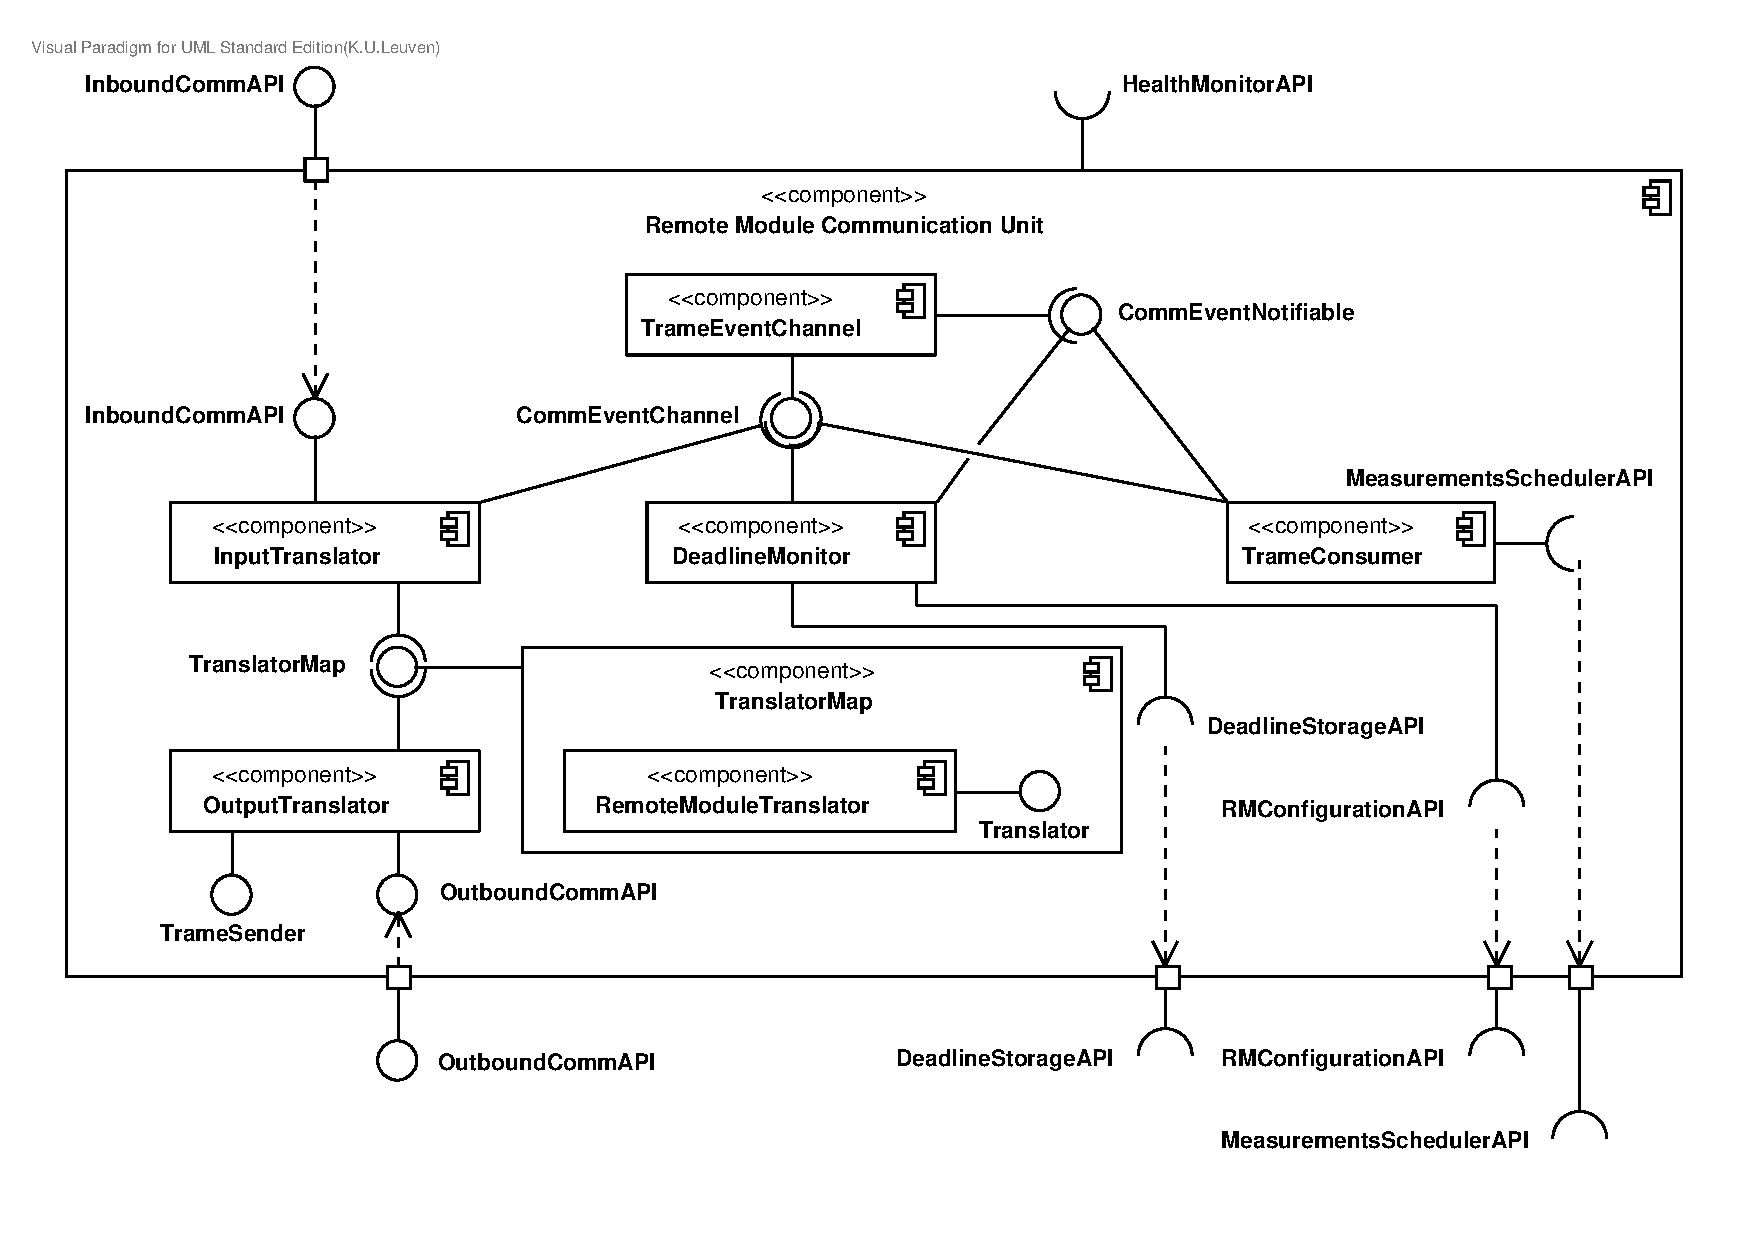
\includegraphics[width=\textwidth]{figs/add-it2-interfaces.pdf}
		\caption{Overview of the interfaces and components in the remote
		module communication unit}
		\label{fig:it2/interfaces}
	\end{centering}
\end{figure}

\subsection{Step 5: Verify and refine}
\label{add:it2/verification}

\npar All the drivers were resolved so no futher decomposition of any of these
modules has to take place because there are no more requirements to divide
amongst the components. 
